%!TEX root = ../_thesis.tex
\chapter{Conclusion and Discussion} % (fold)
\label{c-conclusion}
% Resumen resultados itemizados

During this work, we have explored with distinct  complementary experimental and computational  approaches the sequentiallity in the neuronal dynamics, from the sequential activation of ionic channels in the generation of action potentials, to the cycle-by-cycle dynamics in CPG circuits. Here is a summary of the main results presented in this thesis (see also Fig. \ref{fig:discussion summary}):

\begin{itemize}
	\item Part 1: Sequential dynamical invariants.
 \begin{itemize}
     \item We have illustrated the importance of the study of neuronal sequential dynamics at different description levels.
     \item We have hinted the universality of sequential dynamical invariants by showing their  presence in the feeding CPG of  \textit{Lymnaea stagnalis} both in experimental and modeling data, i.e., in a different animal model from the one used in the work that reported their discovery.
     \item We have shown that dynamical invariants can be found in models when the circuit displays enough cycle-by-cycle variability, which can be induced by an external stimulus.
     \item The models that simulated the variability under the stimulation of specific neurons predicted that the dynamical invariants change depending on the neuron stimulated. This prediction was validated experimentally.
     \item Dynamical invariants are indicators of the functional distribution of  variability  in the CPG.
     \item Neural intrinsic variability in models is usually limited but crucial to study the sequential variability in neural dynamics.
     \item It is possible to study the functional role of sequential dynamical invariants by using  the robust linear relations of neural sequence intervals to control the motor coordination of a hybrot.
 \end{itemize}
	\item Part 2: CW-NIR laser illumination as an effective modulatory technique.
     \begin{itemize}
         \item Sustained CW-NIR laser illumination asymmetrically accelerates action potential dynamics and the spiking rate on single neurons.
         \item The preliminary results in electrically coupled neurons (a minimal circuit) show the potential of CW-NIR to modulate circuit dynamics.
         \item    Modifying the wavelengths of the CW-NIR laser can evoke different changes in action potential metrics. The results illustrate the importance of selecting  wavelenght, power and duration for a specific modulation goal.
         \item A model study of the effect of CW-NIR showed that no biophysical candidate alone could fully reproduce the observed modulation and the global modulation through temperature change was the closest approximation to it.
         \item The closed-loop protocol unveiled the CW-laser effect at different phases of the neuron dynamics, showing a different modulation depending on the instant of illumination.
         \item The code of this closed-loop protocol was published in open-access and can be easily generalized for other neuron types and research contexts.
     \end{itemize}
\end{itemize}
\begin{figure}[htb!]
	\centering
%	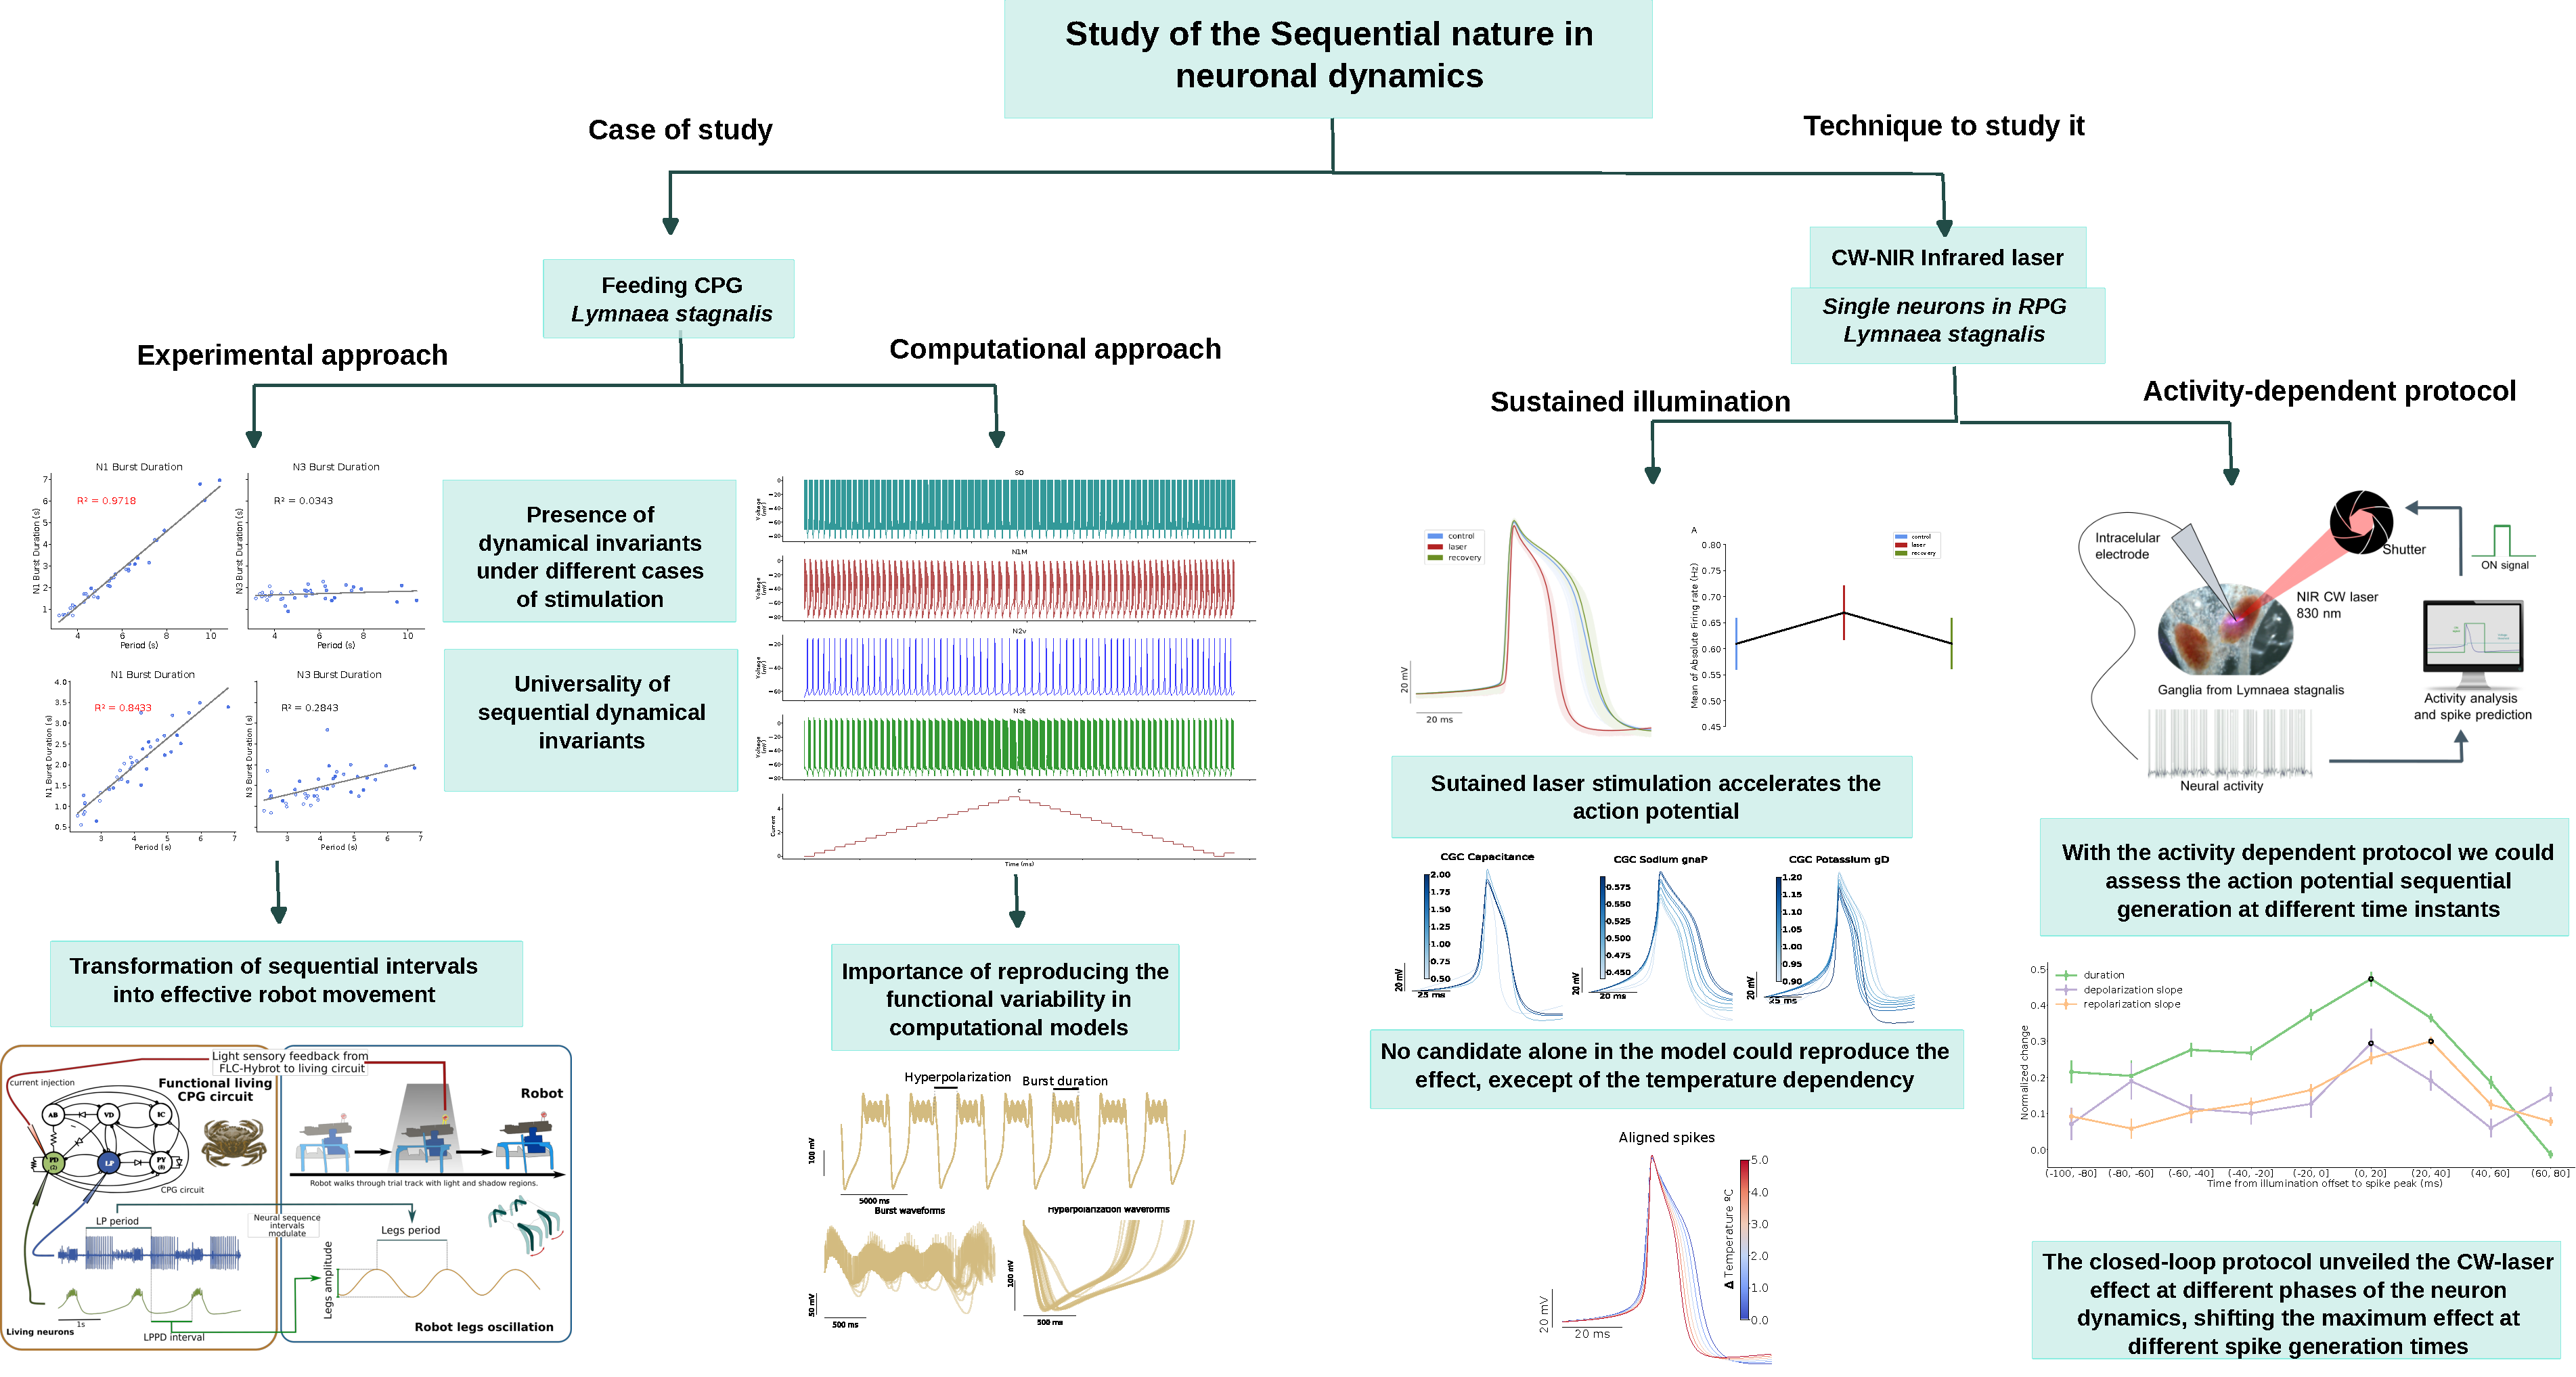
\includegraphics[width=0.9\textwidth]{img/panel discussion.pdf}
	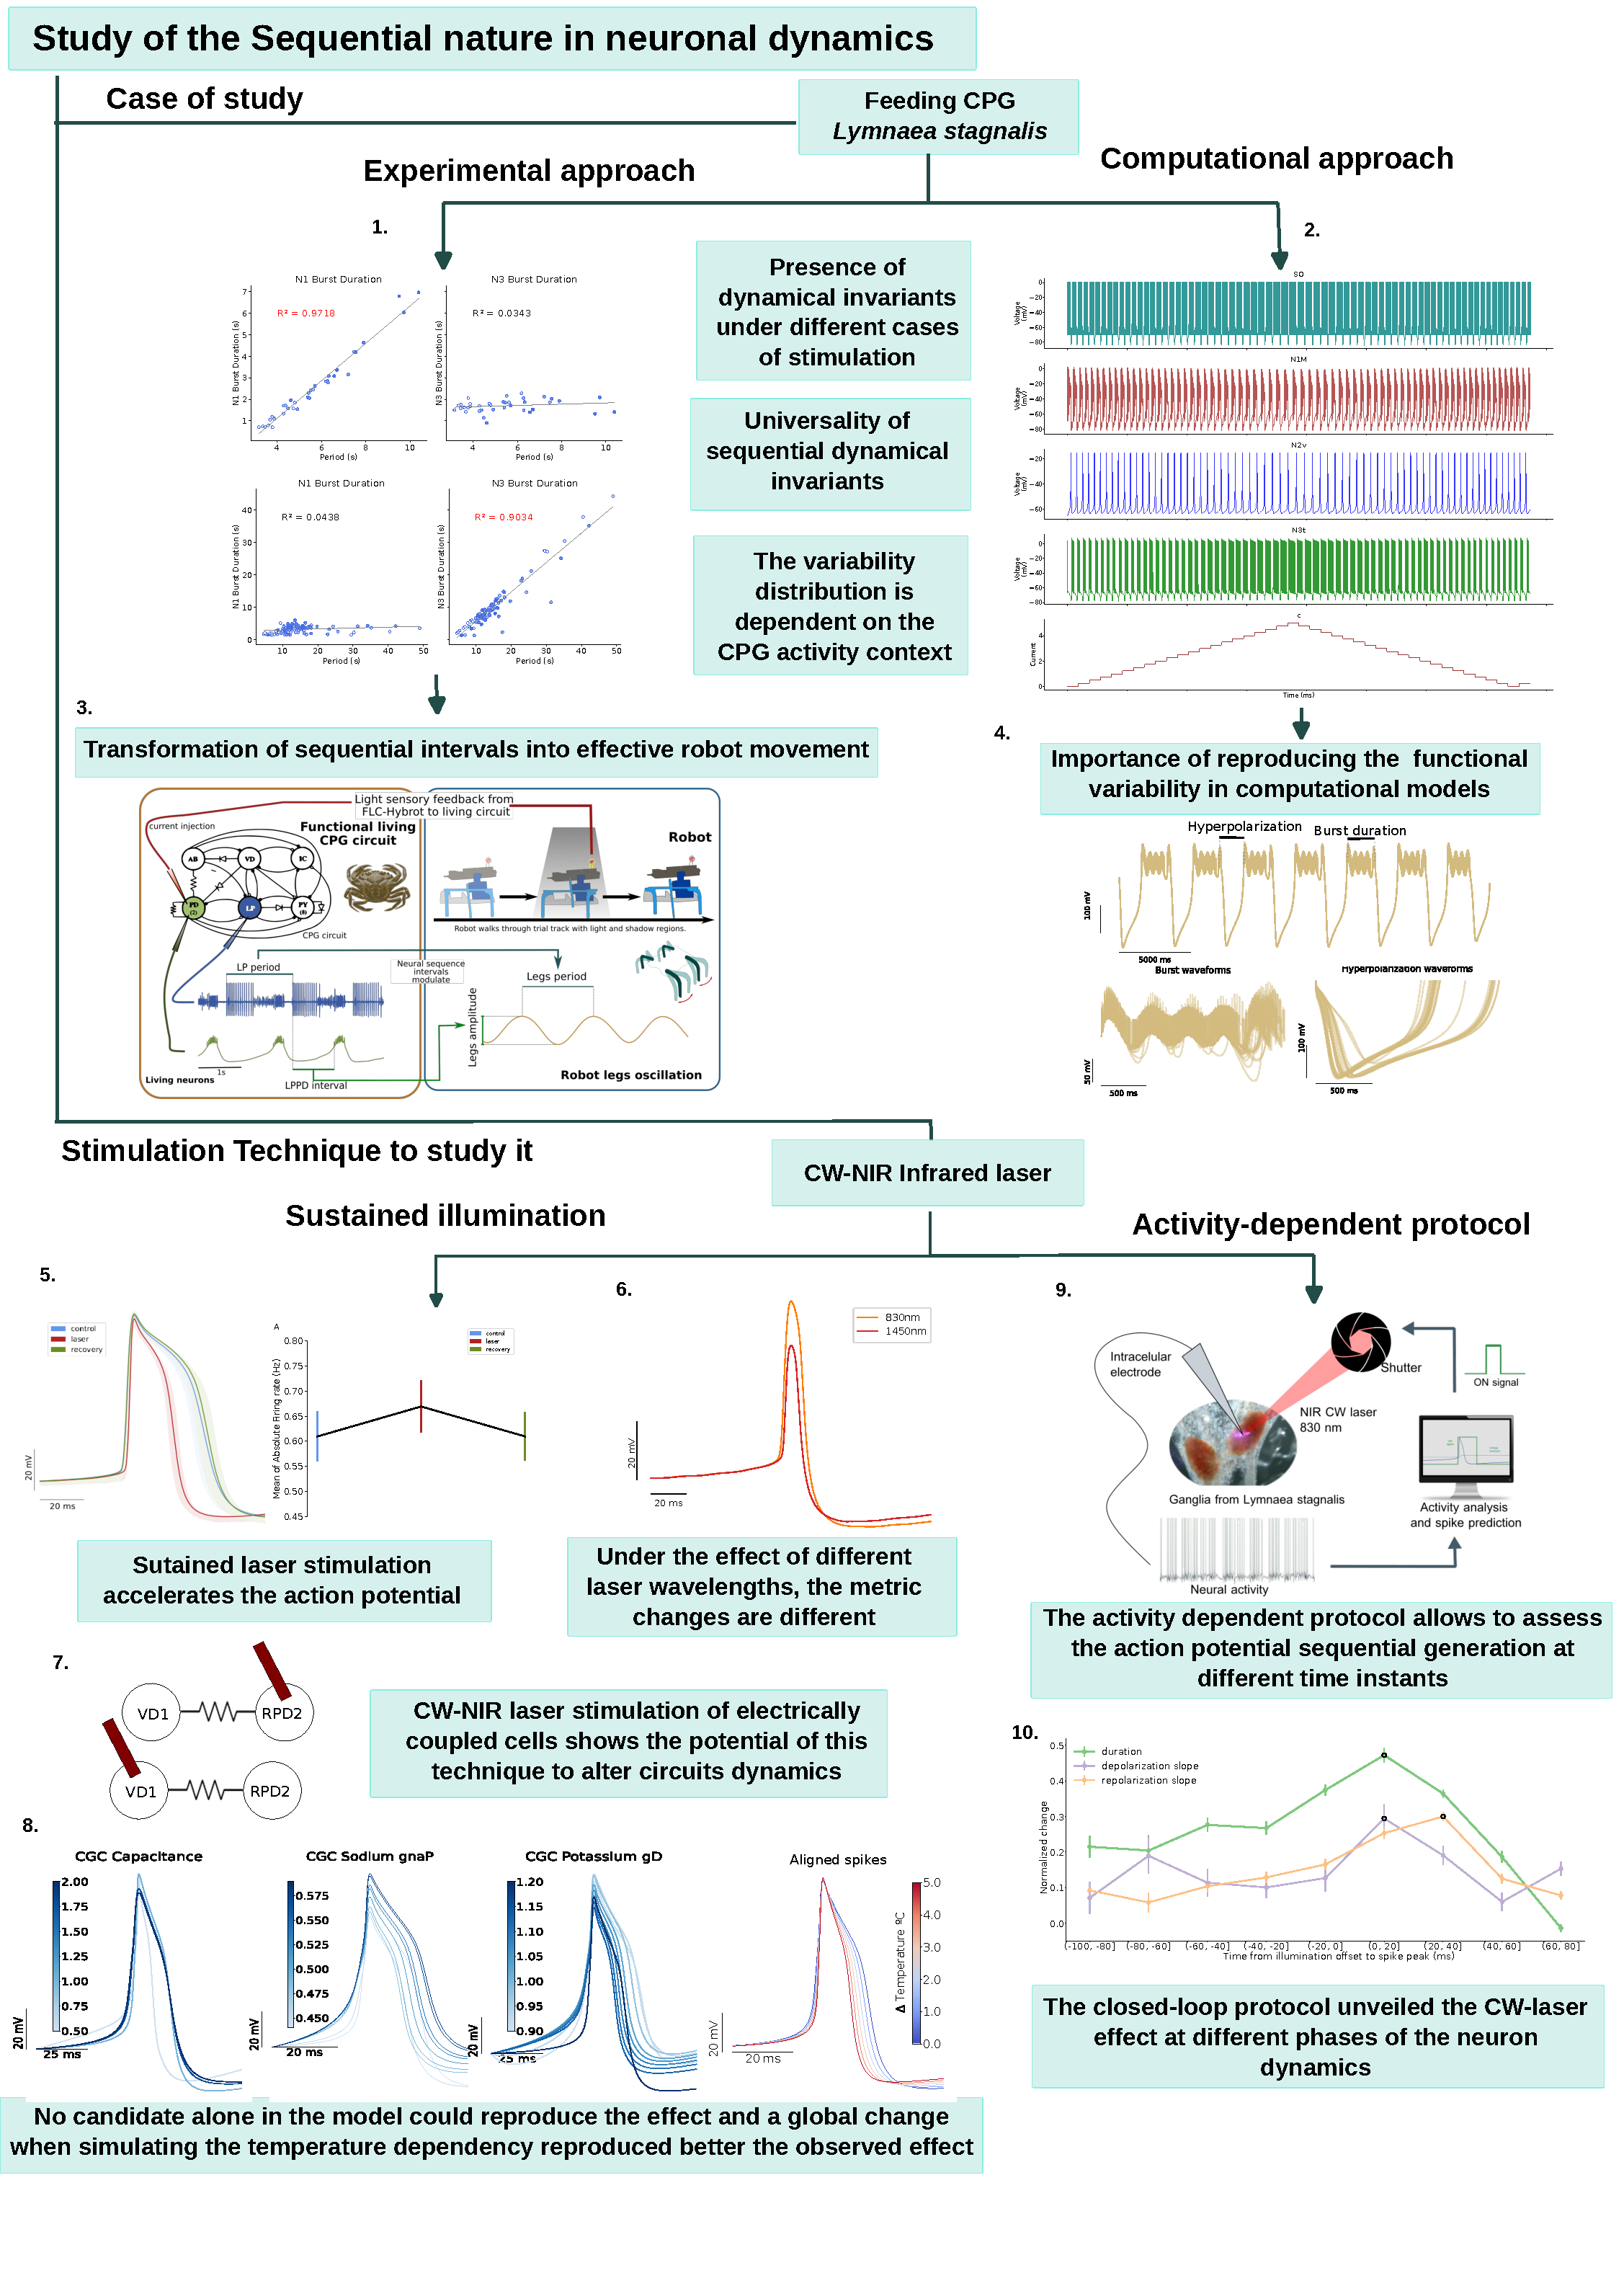
\includegraphics[width=0.75\textwidth]{img/panel_discussion_vertical_figures.pdf}
	\caption{Schematic summary of the results presented in this work. In the feeding CPG of \textit{Lymnaea stagnalis} we explored in (1) experimental and (2) computational data the presence of dynamical invariants (Secs. \ref{sec:experimental sussex} and \ref{c-invariants-model}), showing strong linear relations and associating this to the possible functional role of this indicator. The experimental results were complemented exploring the transformation of (3) robot movement into effective robot movement maintaining strong linear relations (Sec. \ref{sec:robot}). We also showed the (4) importance of reproducing the functional variability in computational models (Sec. \ref{sec:model variability}. As a way to modulate neural dynamics we characterized the effect of the CW-NIR laser in single neurons in a sustained and activity dependent protocol. We showed that (5) the spike waveform is modified during the laser illumination, as well as the firing rate (Sec. \ref{sec:sustained effect}), and discussed the effect at (6) different wavelengths (Sec. \ref{subsec:wavelengths}). We showed also (7) preliminary results in the stimulation of a minimal circuit (Sec. \ref{subsec:electrical}). The computational model analysis (8) revealed the combination of candidates to reproduce the effect and the importance of the temperature role (Sec. \ref{sec:laser models}). (9) The activity-dependent protocol (10) allowed to assess the action potential generation at different phases (Sec. \ref{sec:activity dependent}).}
	\label{fig:discussion summary}
\end{figure}

	
In chapter \ref{c-invariants}, we analyzed the sequential dynamical invariants in a CPG circuit. The goal was to prove the hypothesis presented in \textcite{elices_robust_2019} that the strong linear relationships found between some cycle-by-cycle intervals in the pyloric CPG of the \textit{Carcinus maenas} were not a specific feature of that particular CPG, but a general phenomenon for effective autonomous motor coordination. Thus, the first result showed in \ref{c-invariants} was \textbf{the universality of sequential dynamical invariants}, found also in the feeding CPG of \textit{Lymnaea stagnalis}. We proved this showing their presence not only in a detailed model of the circuit, but also in experimental recordings of the CPG. In the model, we quantified the variability induced by a ramp-current in specific neurons. We explored the variability and the correlations between period and the different intervals in the cycle showing the presence of sequential dynamical invariants.  \textbf{The variability distribution and, consequently, the sequential dynamical invariants change as the neuron stimulated in the model simulation changes}. This highlights the importance of the balance between robustness and flexibility of the sequences for motor coordination through the relation between the neurons in the circuit dynamics. The constrained variability allows an autonomous cycle-by-cycle adaptation. Thus, the computational model configuration and the resulting dynamics must reach a minimum degree of variability in the simulations for the emergence of sequential dynamical invariants. We supported these results analyzing different recordings from neurons in the buccal ganglion, that represented the circuit. We discussed in that chapter the difficulties defining the three phases of the feeding CPG in comparison with the pyloric CPG. Thus, after identifying the three phases of the circuit based on combination of interneurons and motoneurons signals, we analyzed the variability and relations between intervals cycle-by-cycle for spontaneous activity cases and current stimulation driven activity in electrophysiological recordings. We showed the intervals variability and relations in examples of spontaneous activity and \textbf{found sequential dynamical invariants in this spontaneous neural activity.} We also analyzed different cases of stimulation, first SO driven stimulation, spontaneously and by induced stimulation, and reproduced the results in the model, \textbf{showing a change in the variability distribution when the rhythm is modulated by SO.} From this premise that the rhythm is different as the source varies, we analyzed cases where the rhythm was modulated by CV1a neuron stimulation and by MLN nerve. In both cases, \textbf{the interval variability was distributed between N1 and N3 phases}.

Based on these experimental and theoretical results, we also presented in \ref{c-invariants} a study on neural variability. In the modeling side, \textbf{we analyzed the importance of variability in the study of neuronal dynamics and the limitation of classical models to reproduce the intrinsic functional variability of neurons}. We compared different examples of neural activity in living and modeled neurons and their variability, \textbf{ showing the model limitations}. Regarding the experimental approach, we explored the possibility of translating the sequential intervals into effective robot movement. This is important in order to explain the functional meaning of the strong relationships that we observed in specific intervals, which as we discussed is related to the context and the source of the rhythm. In this first prototype, \textbf{we demonstrated that it is possible to achieve an effective robot movement in a robot maintaining strong cycle-by-cycle linear relations}.

In the study of the sequentiality in CPGs, we saw the importance of using effective tools to alter the spontaneous neural activity noninvasively. In chapter \ref{c-laser} \textbf{we explored in detail the CW-NIR laser as a stimulation technique experimentally, theoretically and in activity-dependent protocols}. First, we show the effect of illuminating single cells and how \textbf{CW-NIR sustained illumination asymmetrically accelerates action potential dynamics and increases the firing rate on single neurons.} We tested the effect of the laser stimulation in a minimal circuit by \textbf{illuminating electrically coupled neurons, showing that the main modulation was in the illuminated neuron, slightly modifying the coupled neuron that did not receive the laser stimulation}. We also showed the preliminary results of the wavelength-effect relation, analyzing the laser effect in spike duration, amplitude and slopes with different laser wavelengths and powers, \textbf{showing a modulation of the amplitude as the laser wavelength and power increases that is not showed at low-wavelengths values.} This experimentally observed effect was dissected through model simulations, exploring the possible candidates: ionic channels and capacitance, in conductance-based models, with and without temperature dependence description, showing that \textbf{no candidate alone could fully reproduce the observed modulation and that the global modulation through temperature change was the closest approximation to it.} Finally, \textbf{we presented a closed-loop protocol to alter the action potential at distinct sequential generation phases that can be generalized for distinct subjects and neurons}. With this stimulation protocol \textbf{we unveiled the CW-laser effect at different phases of the neuron dynamics,  identifying different spike waveform changes depending on the time instant of the illumination} We also supported this results with \textbf{a model simulation, tuning some of the channels only at depolarization and repolarization phases, showing the enhancement of the effect as the stimulation time changes.}

The study of temporal restrictions in the sequential activation of motor circuits can have strong implications in neurorrehabilitation and in the understanding of the brain processing of the motor activation. This can unveil the key aspects of the relation between neural variability, robust sequentiality and flexibility in motor control that is observed in living systems, such as in CPGs. For this, it is necessary to expand the study of sequential neural  variability in different animals but also to relate the sequential dynamical invariants to their role in the motor output, relating their activation to different contexts. These restrictions can be indicators of the state of the system and can be associated to the importance of modulating each phase at the current moment, e.g., protraction phase in the presence of food is crucial to achieve the food ingestion as in the MLN stimulation example, while its role when the circuit is active in the absence of food it is not that important, so the variability can be distributed differently, as it was the case of the spontaneous activity with a high-correlation of N3 to the period. In this direction, it is important to improve the intrinsic variability in model simulations by an extended description of chaotic dynamics of the neural activity and its expansion to more complex circuits and systems. The study of the time-interval restrictions in living circuits that produce and ensure the sequential dynamical invariants can also be translated into the design of robots with the robust motor coordination observed in CPGs. These examples will be of high interest for applications in neurotechnology and autonomous robotics design. 

The laser stimulation can help to further explore this dynamics by the effective modulation. The study of this novel neuromodulatory technique might have strong implications for both research and clinical applications by its noninvasive nature. Laser stimulation has been gaining ground in the field of optical stimulation, often implemented as long-wavelength pulsed laser stimulation. It is important to validate different stimulation options such as the sustained continuous-wave and activity-dependent stimulation, of high interest for personalized treatments. The protocol presented in this work might be enhanced with a larger temporal precision, down to the nanosecond scale. This will be relevant to extrapolate it to different systems, regardless of their neural activation time scale, but also to dissect precisely the ionic channel activation dynamics. Furthermore, a in-deep characterization of the laser illumination and its safety range of activation will be of great importance for developing future clinical applications. In this work, we showed a strong and reversible effect, that did not damage the neurons illuminated, which indicates the power used could be increased. A precise characterization of the power tolerated by the neurons would set the safety ranges of its application. The preliminary study of the wavelength-effect relation showed the importance not only of the power, but also that of the laser wavelength in terms of the effect produced, so the analysis of the relation of the wavelength might expand this range of applications but also distinguish between other different mechanisms such as photo-electrical, photo-thermal, etc. A future line of study would also assess the effect of CW-NIR laser in circuits, based on the preliminary results, it should be possible to modify the neurons in a circuit by the stimulation of one of its neurons. This could be studied in CPG circuits, as in the case of the feeding CPG, by illuminating neurons that have an activation/modulatory role in the circuit, such as the CGC neuron in the cerebral ganglion, away from the buccal ganglion but connected to it. Finally, as discussed in this work and laser neurotechnology literature, a photo-thermal effect is one of the main actuators behind the neuronal laser stimulation, however with the current tools and techniques it is not possible to have a detailed description of the change of temperature in the cell. In this line, although the preliminary results were not included in this work, we have explored the possibility of a more precise estimation of the temperature change using silver nanoparticles. These particles could be directly on the membrane, reducing the area of temperature change measurement, and the variation of temperature could be estimated by their irradiation. This precise measurement of the temperature could also help improve the model simulations, with the specific change in the neurons. Also exploring the fast change observed in the activity-dependent protocol with a small change in temperature according to the pipette estimation, can help understand the source of the effect.

The study of neural sequences at multiple spatial and temporal scales can provide novel insights to relate neural dynamics and behavior. Novel neurotechnologies can contribute to identifying and exploiting the sequential nature of neural information processing. The results discussed in this thesis in the context of neural sequences can also have strong implications in the field of neurorrehabilitation, robotics, and artificial intelligence derived from the understanding of sequential dynamical invariants. 

% 7.2 Activity-dependent stimulation in the nanoseconds scale
% 7.3 Safety values of CW-NIR stimulation 
% 7.4 Temperature change in neurons estimation using silver nanoparticles


% Implicaciones de los resultados
% Trabajo futuro

